% ********** Rozdział 1 **********
\chapter{Opis struktury projektu}
\section{Diagram Klas}
\begin{figure}[h]
    \centering
    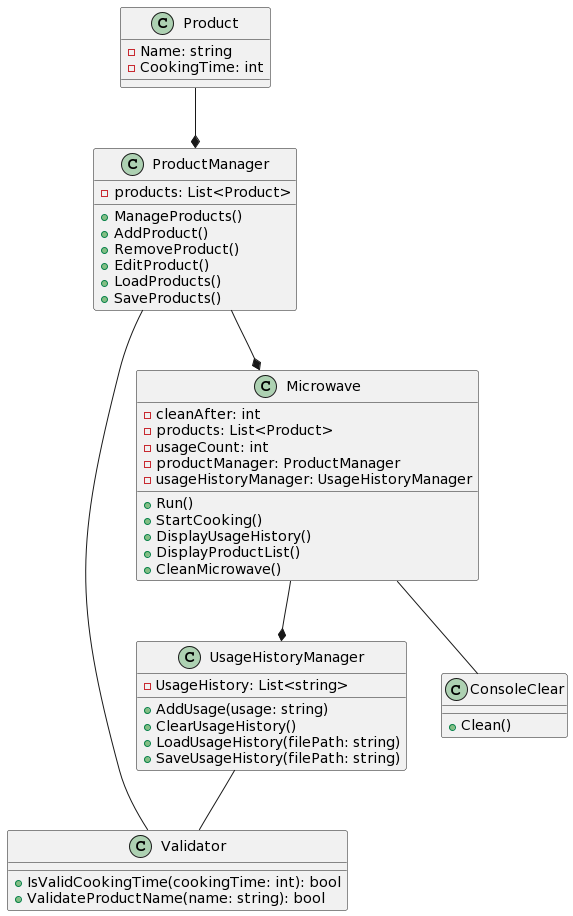
\includegraphics[width=0.7\textwidth]{Diagram.png}
      \caption{Diagram Klas - Opis projektu}
    \label{fig:example}
\end{figure}

\newpage

\section{Opis Diagramu Klas}

Diagram klas przedstawia system kuchenki mikrofalowej. Składa się on z klas oraz relacji między nimi.

\subsection{Klasy}

\begin{itemize}
  \item \textbf{Product}: Klasa reprezentująca produkt, który może być podgrzewany w mikrofalówce. Posiada właściwości Name (nazwa produktu) i CookingTime (czas podgrzewania).
  \item \textbf{ProductManager}: Zarządza produktami dostępnymi w mikrofalówce. Posiada listę produktów oraz metody do dodawania, usuwania, edycji, ładowania i zapisywania produktów. Wykorzystuje walidację produktów za pomocą klasy Validator.
  \item \textbf{Validator}: Klasa narzędziowa do walidacji danych, takich jak poprawność czasu podgrzewania i nazwy produktu.
  \item \textbf{Microwave}: Główna klasa reprezentująca mikrofalówkę. Zarządza procesem gotowania, wyświetlaniem historii użycia, zarządzaniem produktami, czyszczeniem mikrofalówki i diagnostyką.  Wykorzystuje obiekty klas ProductManager, UsageHistoryManager i ConsoleClear.
  \item \textbf{UsageHistoryManager}: Zarządza historią użycia mikrofalówki. Przechowuje listę zdarzeń użytkowania, z możliwością dodawania, czytania, czyszczenia, ładowania i zapisywania historii.
  \item \textbf{ConsoleClear}: Klasa narzędziowa do czyszczenia konsoli po zakończeniu operacji.
\end{itemize}


\subsection{Relacje}

\begin{itemize}
  \item Klasa Product jest wykorzystywana przez ProductManager, który zarządza nimi.
  \item ProductManager korzysta z klasy Validator do walidacji danych produktu.
  \item Microwave wykorzystuje ProductManager do zarządzania produktami, korzysta z UsageHistoryManager do zarządzania historią użytkowania, ConsoleClear do czyszczenia konsoli po zakończeniu operacji.
\end{itemize}
% ********** Koniec rozdziału **********
